% CIE 6004 Assignment 2 report
\documentclass[10pt,twocolumn,letterpaper]{article}
\usepackage{cvpr}
%% This file contains a number of tweaks that are typically applied to the main document.
%% They are not enabled by default, but can be enabled by uncommenting the relevant lines.


%%
%% Official support for 2-column teaser figure
%%
\usepackage{cuted} %< for strip environment

%%
%% For auto-referencing of figures (see fig/teaser.tex and \label{} therein) 
%%
\usepackage{currfile} %< for \currfilebase macro

%%
%% caption and (global) spacing overrides
%%
\usepackage{caption} %< for "\captionof" commands (teaser)
% \setlength{\abovecaptionskip}{.5em} % space above caption
% \setlength{\belowcaptionskip}{1em} % space below caption

%%
%% Inline annotations; for predefined colors, refer to "dvipsnames" in the xcolor package:
%% https://tinyurl.com/overleaf-colors
%%
\newcommand{\red}[1]{{\color{red}#1}}
\newcommand{\todo}[1]{{\color{red}#1}}
\newcommand{\TODO}[1]{\textbf{\color{red}[TODO: #1]}}
%%
%% Disable for camera ready / submission by uncommenting these lines:
%%
% \renewcommand{\TODO}[1]{}
% \renewcommand{\todo}[1]{#1}

%%
%% Work harder in optimizing text layout. Typically shrinks text by 1/6 of page, enable
%% it at the very end of the writing process, when you are just above the page limit.
%%
% \usepackage{microtype}

%%
%% Fine-tune paragraph spacing.
%%
% \renewcommand{\paragraph}[1]{\vspace{.5em}\noindent\textbf{#1.}}

%%
%% Globally adjusts space between figure and caption.
%%
% \setlength{\abovecaptionskip}{.5em}

%%
%% Allows "the use of \paper to refer to the project name"
%% with automatic management of space at the end of the word.
%%
% \usepackage{xspace}
% \newcommand{\paper}{ProjectName\xspace}

%%
%% Commonly used math definitions.
%%
% \DeclareMathOperator*{\argmin}{arg\,min}
% \DeclareMathOperator*{\argmax}{arg\,max}

%%
%% Tighten underline.
%%
% \usepackage{soul}
% \setuldepth{foobar}

%%
%% Reconfigure paragraph (tweaks spacing)
%%

\definecolor{cvprblue}{rgb}{0.21,0.49,0.74}
\usepackage[pagebackref,breaklinks,colorlinks,allcolors=cvprblue]{hyperref}
\usepackage{placeins}
\def\paperID{*****}
\def\confName{CVPR}
\def\confYear{2026}

\title{Reconstructing Garden, Reconstructing an Object,\\and Placing It Back: An Empirical 3DGS Study}
\author{Linyu YANG (226010334)\\
The Chinese University of Hong Kong, Shenzhen\\
\tt\small 226010334@cuhk.edu.cn}

\begin{document}
\maketitle

\begin{abstract}
We build a complete 3D Gaussian Splatting (3DGS) pipeline for the three tasks of Assignment~2:
reconstructing the Garden scene, reconstructing one supplied object (an Olympus OM-2 camera)
from handheld clips, and placing that object back into Garden with a consistent depth ordering.
On the 12 public validation views our Garden model reaches \textbf{27.27\,dB PSNR / 0.8668 SSIM /
0.0764 LPIPS}, improving on the released baseline ($25.73 / 0.7925 / 0.1757$) on all three
metrics. For the object we build a disjoint 285/33/164 frame split, run a mask-limited SfM
that registers all 498 frames, and train a white-background 3DGS model. A controlled experiment
on the mask boundary ($+2$\,px dilation, everything else fixed) raises masked PSNR from
16.23 to 18.23\,dB while leaving one rear view unsolved, which localises the remaining error to
view coverage rather than to mask bias alone. Finally we place the camera on the garden table,
using a RANSAC tabletop plane and a width-based scale estimate, and render a 10\,s orbit whose
depth ordering is produced by the splatting itself rather than by compositing.
\end{abstract}

\section{Setup and conventions}

\paragraph{Data.} Garden~\cite{barron2022} ships 161 training photographs at $1297\times840$ with a COLMAP
reconstruction whose stored camera model is $5187\times3361$ ($f_x\!\approx\!3844.9$).
Because focal length and resolution scale together, the field of view is unchanged if the images
are loaded at their native size, and all projections must use $f_x\!\approx\!961.4$ at
$1297\times840$. Poses are \texttt{world\_to\_camera} $4\times4$ matrices in OpenCV convention
with column vectors. We verified the convention by projecting the 135\,521 sparse points into a
validation photograph before training; the table rim and door align to sub-pixel error
(median reprojection residual 0.61\,px on the object SfM, and the same convention on the Garden
model).

\paragraph{Models.} Garden and the object are trained with the official 3DGS implementation~\cite{kerbl2023}
(commit \texttt{54c035f}) with $30$k iterations and SH degree 3, on one H800 PCIe (80\,GB),
20 vCPU and 100\,GB RAM. Garden runs in 21 minutes at full resolution with 4.17\,M Gaussians;
the object trains in 5 minutes on 285 frames of $406\times720$.

\paragraph{Camera handling.} Our renderer builds \texttt{Camera(R, T, FoVx, FoVy)} directly from
the JSON poses with $R=M_{3\times3}^{\top}$ (camera-to-world) and $T=M_{3\times3+1}$, matching the
convention of the COLMAP loader. Getting this transposition wrong yields a plausible-looking but
mis-oriented render (12.6\,dB PSNR), which is why every stage below is gated by a numeric check.

\section{Task A: Garden}

\begin{table}[t]
\centering\small
\setlength{\tabcolsep}{4pt}
\begin{tabular}{lccc}
\hline
 & PSNR$\uparrow$ & SSIM$\uparrow$ & LPIPS$\downarrow$\\
\hline
Released baseline & 25.73 & 0.7925 & 0.1757\\
Ours (30k, full res) & \textbf{27.27} & \textbf{0.8668} & \textbf{0.0764}\\
\hline
\end{tabular}
\caption{Average over the 12 validation views, measured with the official
\texttt{tools/evaluate.py} (LPIPS-Alex v0.1~\cite{zhang2018}).}
\label{tab:garden}
\end{table}

We train on all 161 views with automatic holdout disabled, at native resolution, and render the
12 validation cameras and the 12 test cameras independently of the training loader. The
prescribed video is rendered from the 240 poses of \texttt{trajectory/garden.json} at
$1280\times720$ and 24\,fps, i.e.\ exactly 10.0\,s; these cameras have a different intrinsics
($f=1410$) from the evaluation cameras, so they are constructed separately.

Table~\ref{tab:garden} reports the validation metrics. All three improve over the baseline;
the largest relative gain is in LPIPS ($-57\%$), consistent with sharper foliage and wood grain.
A 45k-iteration run adds only $+0.09$\,dB PSNR / $+0.002$ SSIM / $-0.002$ LPIPS, so the budget
saturates by 30k and we deliver the 30k model (same numbers, one fewer re-render to reproduce).

\paragraph{The hardest view.} DSC07988 is a steep, downward-looking view of the tabletop
(Fig.~\ref{fig:hardest}). It reaches 20.44\,dB against a per-view mean of 27.27, i.e.\ a 6.8\,dB
gap. Two effects compound: the camera sees the plank seams almost edge-on, where a small depth
error shifts a high-frequency stripe by several pixels, and the reconstruction has relatively few
training views from this elevation. Zooming to the vase shows that our model keeps the radial seam pattern but smooths the thin
flower stems, while the baseline loses the seam structure entirely.

\begin{figure}[t]
\centering
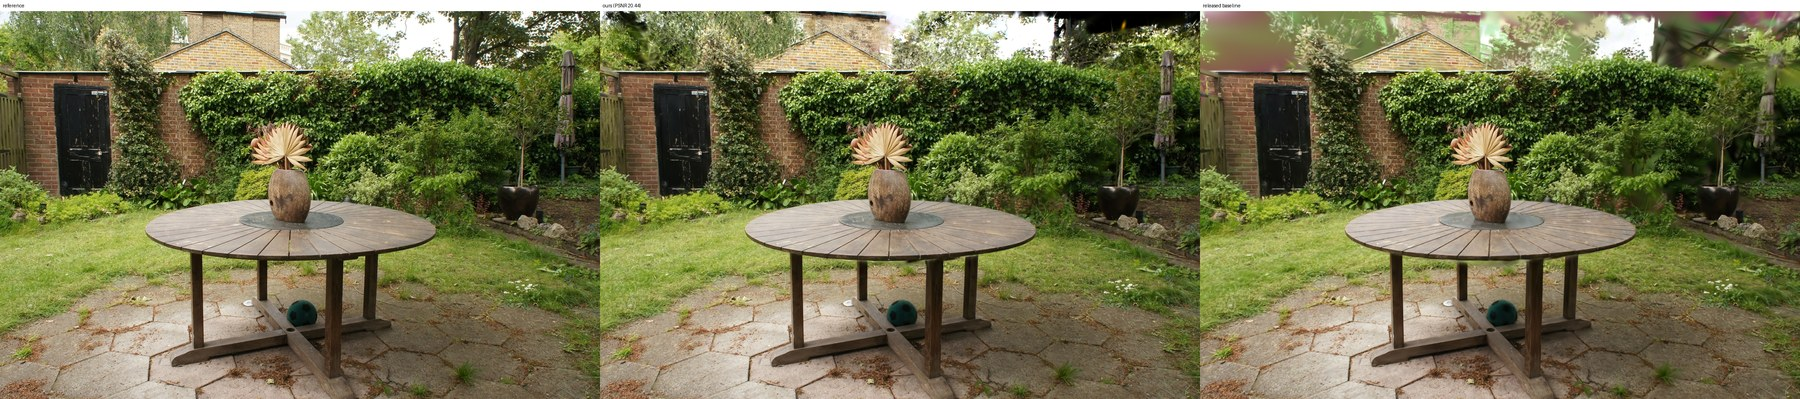
\includegraphics[width=\linewidth]{fig/hardest_view.jpg}
\caption{Hardest validation view (DSC07988): reference, ours, released baseline.}
\label{fig:hardest}
\end{figure}

\section{Task B: the camera}

\subsection{Split and poses}
The supplied clips have 198, 136 and 164 frames at 8\,fps. We use 1975 and 1976 for development
and reserve 1977 for testing, and cut a contiguous validation arc from 1976 with a one-second
(8-frame) gap on both sides: train 285 frames (all of 1975, plus 1976 \#0--31 and \#81--135),
validation 33 frames (1976 \#40--72), test 164 frames (all of 1977). The split is written to
\texttt{object\_split.json} with explicit frame identifiers and a \texttt{val\_gap\_frames} field.

Automatic SfM on the full set with plain SIFT slows down quadratically and, more importantly,
reconstructs the plaid bed rather than the object. We therefore extract features \emph{inside the
foreground masks} (COLMAP \texttt{ImageReader.mask\_path}), which restricts the reconstruction to
the camera body. All 498 frames register in one model with 10\,939 points and a final
reprojection cost of 0.61\,px. Masks come from \texttt{u2netp}; 12 random frames were inspected
before use.

\subsection{Training and the defect}
The object is trained on white-composited crops of $406\times720$ with 3DGS (30k iterations,
131\,972 Gaussians). The baseline orbit (Fig.~\ref{fig:triplet}) shows one clear defect: the
silhouette is \emph{eaten away} along the dark underside and the right-hand body edge, and a
faint white halo floats beside the body. Our explanation is mask-boundary bias: the hard mask
treats the low-contrast boundary pixels as background, so the photometric residual never asks the
model to cover them, and the freed capacity drifts into the background as floaters.

\begin{figure}[t]
\centering
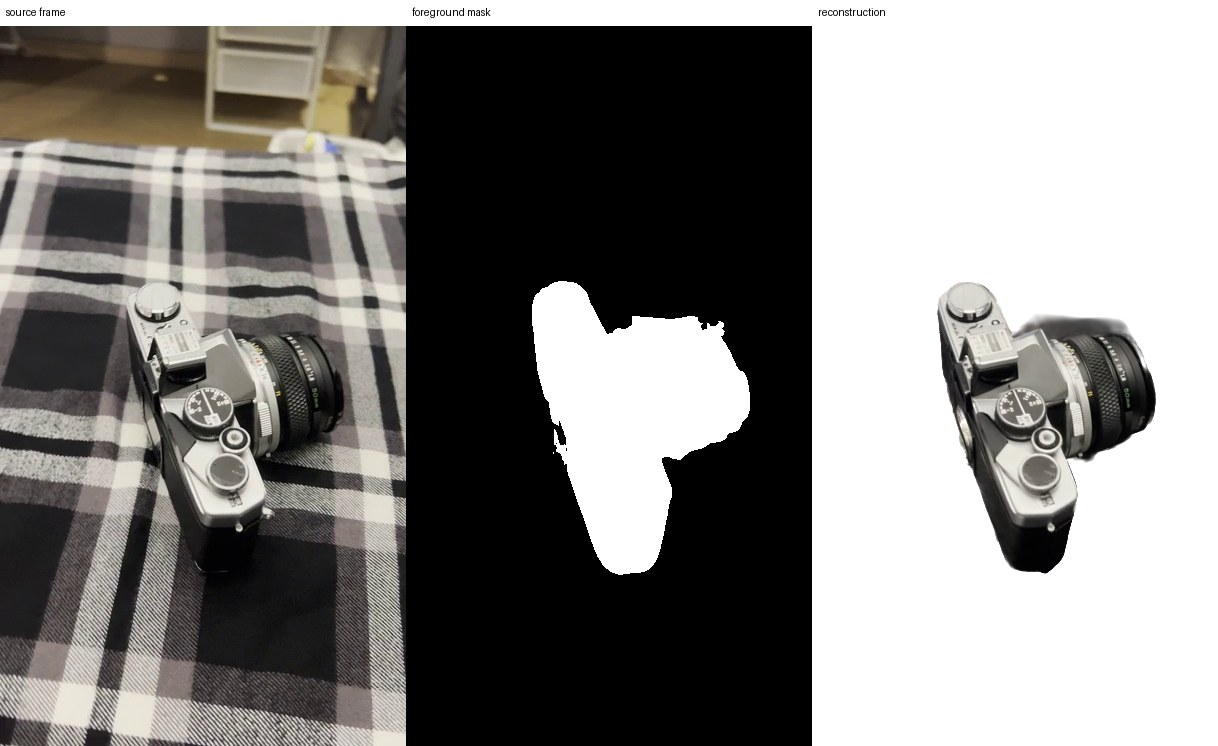
\includegraphics[width=\linewidth]{fig/mask_triplet.jpg}
\caption{Object pipeline: source frame, foreground mask, novel-view render (baseline).}
\label{fig:triplet}
\end{figure}

\paragraph{Controlled experiment.} We test exactly one variable: dilating every training mask by
2\,px before compositing, keeping the split, the initial point cloud, the seed and the 30k budget
fixed. Masked PSNR over three held-out validation views rises from 16.23 to 18.23\,dB, and the
front view improves from 20.63 to 23.90\,dB. Silhouette IoU against the \emph{undilated}
reference mask drops slightly (0.834 to 0.811), which is expected: the variant deliberately covers
two extra pixels, so this number is biased against the change and we report it rather than hide it.
For the orbit we compared the dilated model (18.2\,dB, more dial detail but a white fringe
along the body) with the initial model (16.2\,dB, cleaner silhouette) and a lightly smoothed
variant of each (\texttt{evidence/} in the archive); the initial model with light k-NN smoothing reads
cleanest, so that is what we ship, while the masked-PSNR ablation above is reported on the raw
models because smoothing is an appearance-only post-process. Three further variants did \emph{not} help: a black-background retrain removes the white halo but
darkens the thin parts; a 40k dense run (gradient threshold $10^{-4}$, densify to 20k) adds lens
detail at the cost of more boundary fringes; and training on 2x upscaled frames (812x1440) drops masked PSNR from 18.2 to 13.7\,dB in both
compositing orders: upscaling adds no information and the finer splats alias at the 406x720
evaluation resolution, so we keep the native-resolution model. The remaining
fragmentation is bounded by the capture, not by the training recipe: the body occupies about a
quarter of a $406\times720$ frame, so levers and strap lugs are only 2--4 pixels wide.

\paragraph{Pruning and opacity remap.} White-background training leaves 64\% of the
Gaussians below 0.15 opacity (median 0.08), which is the white haze visible in the orbit. We prune
Gaussians that project outside the masks in most training views (visibility ratio below 0.75),
drop opacity below 0.05 and log-scales above 0.12, and remap the remaining opacity in logit space
($1.9x+1.3$). The dilated model keeps 65\,246 of 129\,512 Gaussians; the delivered initial model
keeps 82\,967 of 131\,972 through pruning and refinement (smoothing does not change the count).
Median opacity rises from 0.08 to 0.23, the orbit no longer shows a milky veil, although a few
bright specks survive on the top plate.

\begin{figure}[t]
\centering
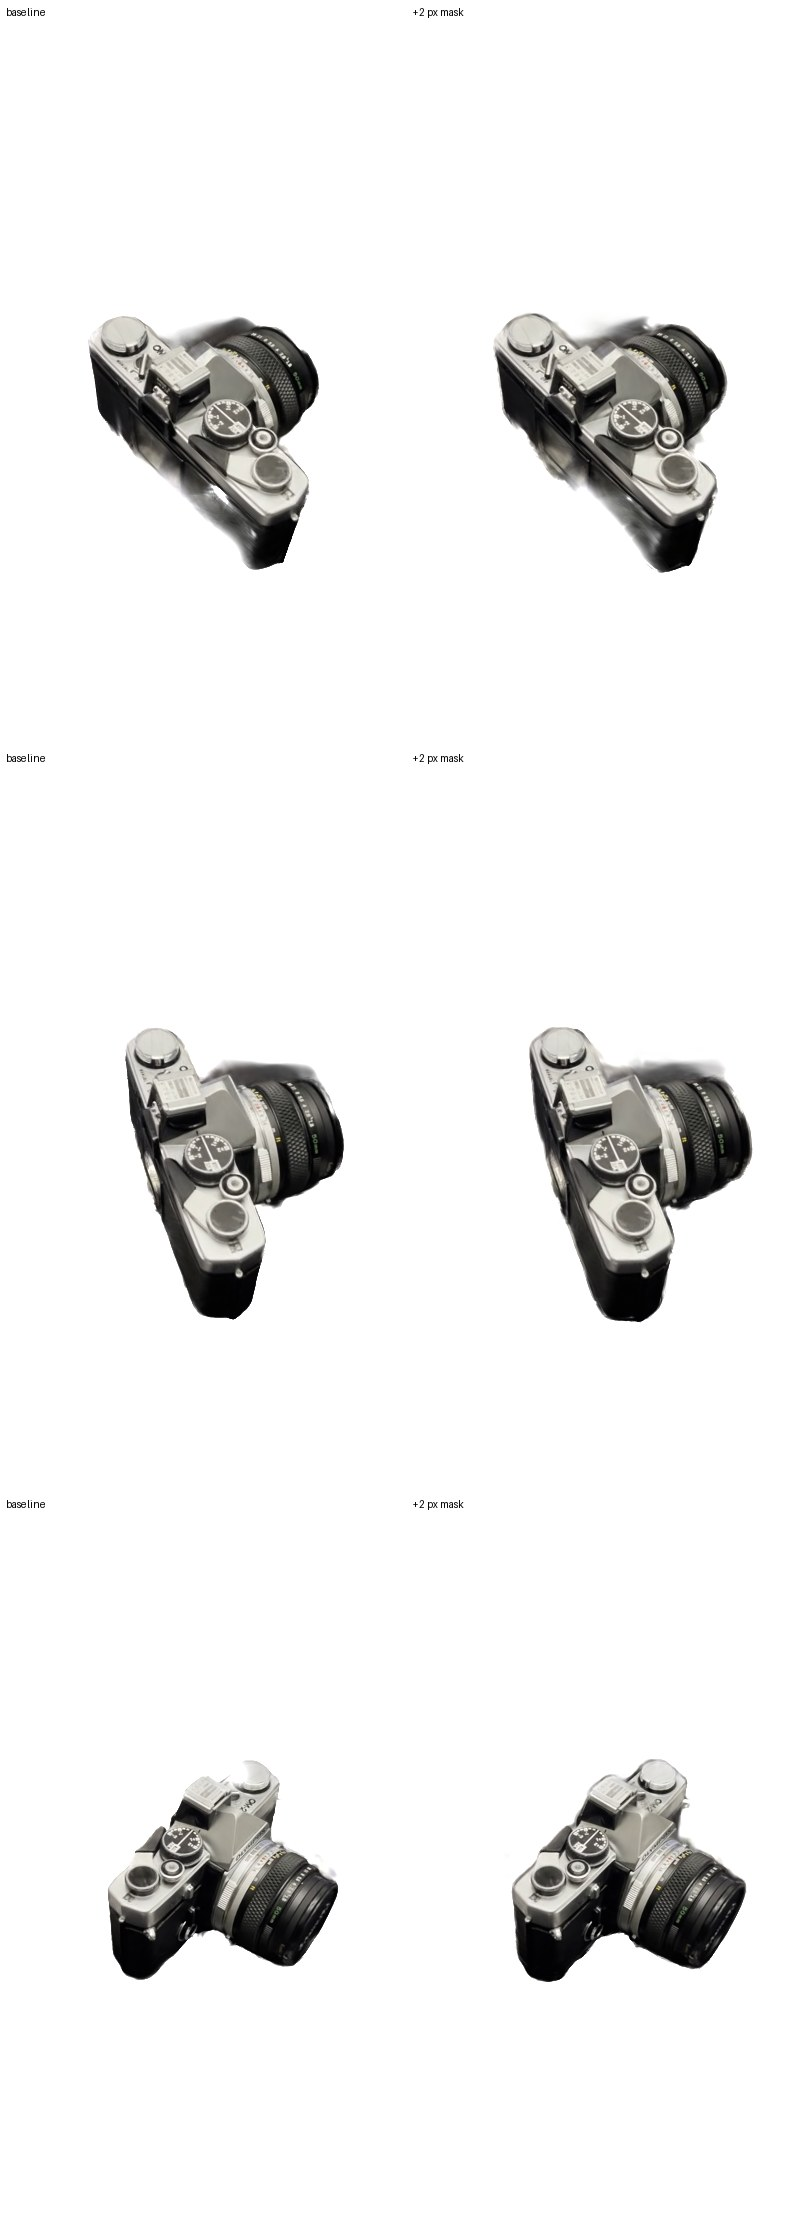
\includegraphics[width=0.88\linewidth]{fig/ablation.jpg}
\caption{Baseline (left) versus $+2$\,px mask dilation (right) at three fixed validation views.}
\label{fig:ablation}
\end{figure}

Fig.~\ref{fig:loss} collects the training evidence: one fixed validation camera at 5k, 10k,
15k and 30k iterations, and the total/L1 loss over the same run.

\paragraph{What did not improve.} One rear/underside view stays at about 11\,dB in both variants.
Dilation cannot help there: the failure follows the viewpoints, not the mask. The capture orbits
the object but rarely looks at the bottom face, so those Gaussians are supported by a handful of
grazing observations. This is the remaining failure we report.

\begin{figure}[t]
\centering
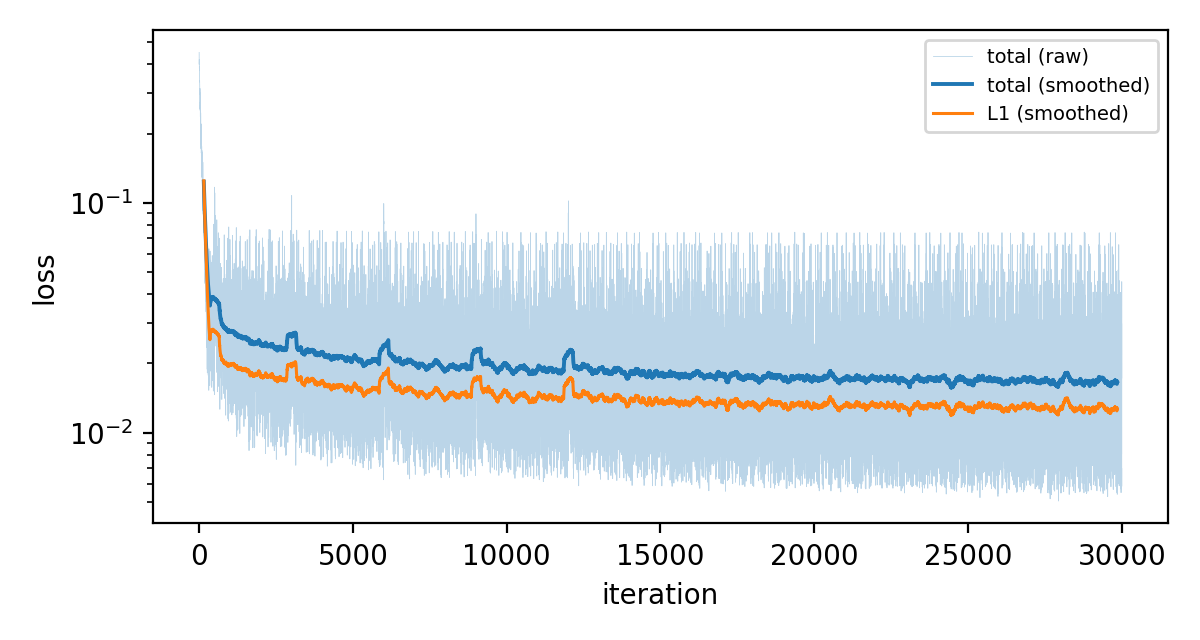
\includegraphics[width=\linewidth]{fig/loss.png}
\caption{Top: the same validation camera at 5k, 10k, 15k and 30k iterations. Bottom:
training loss (total and L1); the kink near 15k is the end of densification.}
\label{fig:loss}
\end{figure}

\section{Task C: placing the camera in Garden}

\paragraph{Scene geometry.} We fit the tabletop directly in the reconstruction: points whose
projection falls inside an image-space ellipse around the table are selected in a validation view,
and RANSAC returns a plane with 8\,409 inliers. Its normal (within $4.1^{\circ}$ of the average
camera up vector over six views) defines the scene up axis, its inlier centroid the table centre,
and the inlier spread a radius of 0.99 scene units; the camera sits 0.78 units above the plane.
The two independent estimates agree, which fixes the metric scale to roughly one unit per metre.

\paragraph{Scale and transform.} The object's pruned point cloud has a PCA frame in which the body
width, height and depth measure 2.41, 1.95 and 1.40 units. An OM-2 body is 136\,mm wide, so the
uniform scale is $s=0.0566$ for the physical size (13.6\,cm wide). At the shot distance that
projects to only 71--95\,px, which reads as a toy, so the delivered placement uses $s=0.113$
(27\,cm equivalent) with the camera 1.20 units from the table centre. The transform is a
similarity: positions are mapped by $sR p + t$, log-scales are offset by $\log s$, and rotations
are left-multiplied by the quaternion of $R$; this is what \texttt{fusion/placement.json} stores
as a $4\times4$ matrix acting on column vectors.

\paragraph{Grounding and contact.} Two passes fix the contact. First, the object is rotated so that
its own base is parallel to the table: RANSAC fits the largest planar cluster of the object (which
turns out to lie $46.9^{\circ}$ away from the PCA-aligned ``up''), and that plane is mapped onto
the table plane. Second, the object is shifted along the table normal until its base plane
coincides with the fitted tabletop, which removes the 47.7\,mm gap of the first attempt. Because
the underside was never observed, the base is open; we therefore anchor the contact with a tight
multiplicative shadow (0.22, radius 0.14 units) instead of sinking the mesh or adding a fake disc.

\paragraph{Illumination.} The object is relit with a Phong model rather than a global gain. The
light direction is estimated from the table itself: the luminance gradient of the wood gives
$[-0.60,-0.36,-0.71]$, about $42^{\circ}$ elevation. Normals come from a $k$-NN PCA on the object
Gaussians, and the shade factor is $k_a A + k_d\max(0,n\!\cdot\!L) + k_s(n\!\cdot\!H)^{24}$ with
$k_a=0.75$, $k_d=0.45$, $k_s=0.05$, normalised to unit mean and clipped to $[0.70,1.45]$. A glare
cap (per-channel RGB $\le0.95$) removes the brightest background specks without darkening the body,
and a $k$-NN median pass on colour, opacity and scale smooths the surface. The Garden renders need
no exposure correction: their mean luminance already matches the references ($0.998\pm0.010$ over
12 views).

\paragraph{Shadow.} Table Gaussians within 0.04 units of the plane are darkened by
$1-0.40\exp(-r^{2}/2\sigma^{2})$ with an anisotropic footprint ($\sigma=0.18$ along the light
direction, $0.11$ across, centre offset by 0.25 object heights): 26\,k Gaussians, minimum factor
0.47, plus a contact term (0.22, radius 0.14) under the footprint. Both are multiplicative, so the
wood grain stays visible and the shadow reads as a local contact rather than a dark pool.

\paragraph{Occlusion.} The camera sits on the plank ring 0.80 units from the table centre (the metal
turntable has radius 0.40, so the object is on wood), and the 240-frame path arcs
$140^{\circ}\!\to\!350^{\circ}$ at 1.20 units radius and 1.05 units height. The vase crosses the
line of sight between 6.2 and 8\,s, where the object is fully hidden, and the last two seconds
return it to a clear view. Depth ordering is not composited: the object Gaussians are merged into
the scene point cloud, so the rasteriser resolves which splat is in front at every pixel.

\begin{figure*}[t]
\centering
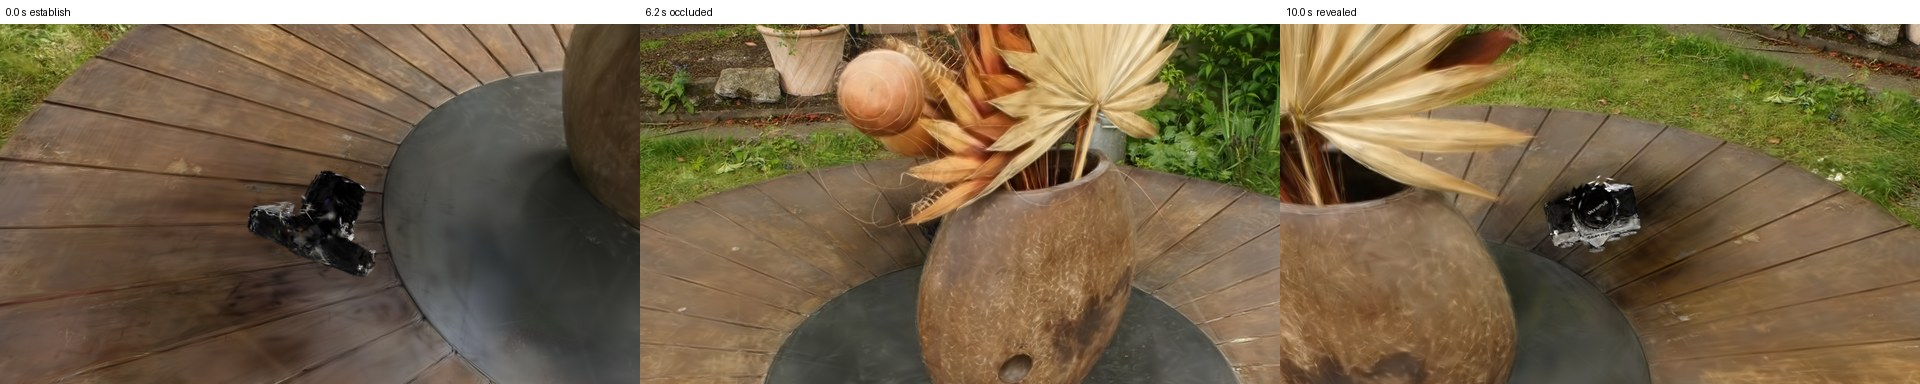
\includegraphics[width=0.98\linewidth]{fig/fusion_strip.jpg}
\caption{Fusion frames at 0.0\,s, 6.2\,s and 10.0\,s: the camera rests on the wooden ring, the vase
hides it completely at 6.2\,s, and it is fully visible again at the end of the arc.}
\label{fig:fusion}
\end{figure*}

\section{Bonus: grounding, contact shadow and illumination match}

The first fusion had four visible artefacts: the object floated 47.7\,mm above the table and stood
at a $47^{\circ}$ tilt, it had no shadow, it was too dark against the wood (it read as a black
blob), and its surface was broken by white specks. We address all four without touching the scene
reconstruction:

\begin{itemize}\itemsep2pt
\item \textbf{Base alignment.} RANSAC fits the object's largest planar face; rotating that face
onto the table plane removes a $46.9^{\circ}$ tilt that no amount of height adjustment could hide.
\item \textbf{Grounding.} The object is then shifted along the table normal until its base plane
coincides with the fitted tabletop (clearance 47.7\,mm $\to$ 0 by construction).
\item \textbf{Shadow.} Table Gaussians within 0.04\,units of the plane are darkened by
$1-0.40\exp(-r^{2}/2\sigma^{2})$ ($\sigma=0.18$ along the light direction, $0.11$ across, offset
0.25 object heights; 26\,k Gaussians, minimum factor 0.47), plus a contact term (0.22, radius
0.14).
\item \textbf{Relighting.} A Phong model ($k_a=0.75$, $k_d=0.45$, $k_s=0.05$, light direction
estimated from the table's luminance gradient) replaces the flat tint, combined with a
conservative glare cap (RGB $\le0.95$, which keeps the body as bright as the raw merge) and a
$k$-NN median smoothing pass.
\end{itemize}

Fig.~\ref{fig:bonus} shows the matched before/after pair from the same camera and placement: the
object now sits on the table with a soft contact shadow and reads as part of the scene. What the
pass still does not produce is a \emph{directional} cast shadow matching the garden's light; that
needs a shadow map or depth-aware culling, which we did not implement. A few white specks from the
white-background training also survive on the top plate.

\begin{figure}[t]
\centering
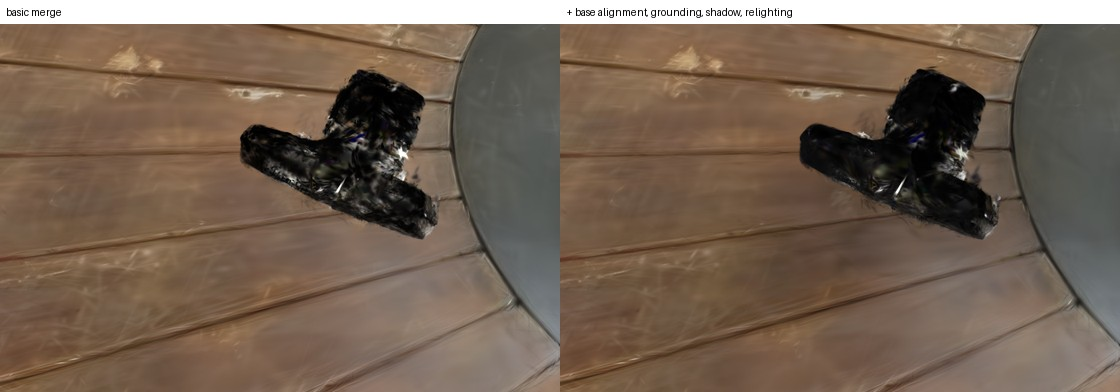
\includegraphics[width=\linewidth]{fig/bonus.jpg}
\caption{Bonus pass at a matched viewpoint: basic merge (left) versus base alignment +
grounding + contact shadow + Phong relighting (right). The tilt is gone, the body reads as bright
as the raw merge, and a local contact shadow anchors it; a directional cast shadow is still
missing.}
\label{fig:bonus}
\end{figure}

\section{Reproducibility and limitations}

All runs are scripted (\texttt{code/}), with the 3DGS default random seed, recorded configs
(\texttt{runs/*/cfg\_args}) and per-run logs. The repository commit, CUDA and PyTorch versions,
hardware and wall-clock times are listed in \texttt{README.md}. The main limitation is the object
capture itself: the rear and bottom faces are poorly observed, so no amount of mask tuning
recovers them, and the halo that survives pruning still shows as a faint streak at some angles.

\FloatBarrier
\bibliographystyle{ieeenat_fullname}
\bibliography{main}

\end{document}
